\section{Introduction}

\begin{frame}
\frametitle{Motivation}
\begin{itemize}
    \item Quantum chemistry calculations are promising early applications of quantum computers
    \item Materials science simulations involve periodic systems and large numbers of atoms
    \item Current focus: Quantum-centric supercomputers with quantum accelerators
    \item Need for hybrid quantum-classical approaches for practical applications
\end{itemize}
\end{frame}

\begin{frame}
\frametitle{Why Quantum Computing for Materials?}
\begin{itemize}
    \item Large solid-state systems require approximations in DFT
    \item Quantum computing can improve accuracy for critical subsystems
    \item Quantum embedding approach similar to QM/MM methods
    \item Potential for better description of electron correlation
\end{itemize}
\end{frame}

\begin{frame}
\frametitle{Our Approach - Core Methodology}
\begin{itemize}
    \item Simplify the problem and consider Aluminum substrate instead of alloys
    \item Approach the problem from DFT simulation workflow
    \item Introduce quantum computer as accelerator to the workflow
    \item Build Hybrid quantum-classical computational framework
    \item Focus on surface-adsorbate interactions
\end{itemize}
\end{frame}

\begin{frame}
\frametitle{Workflow Overview}
\centering
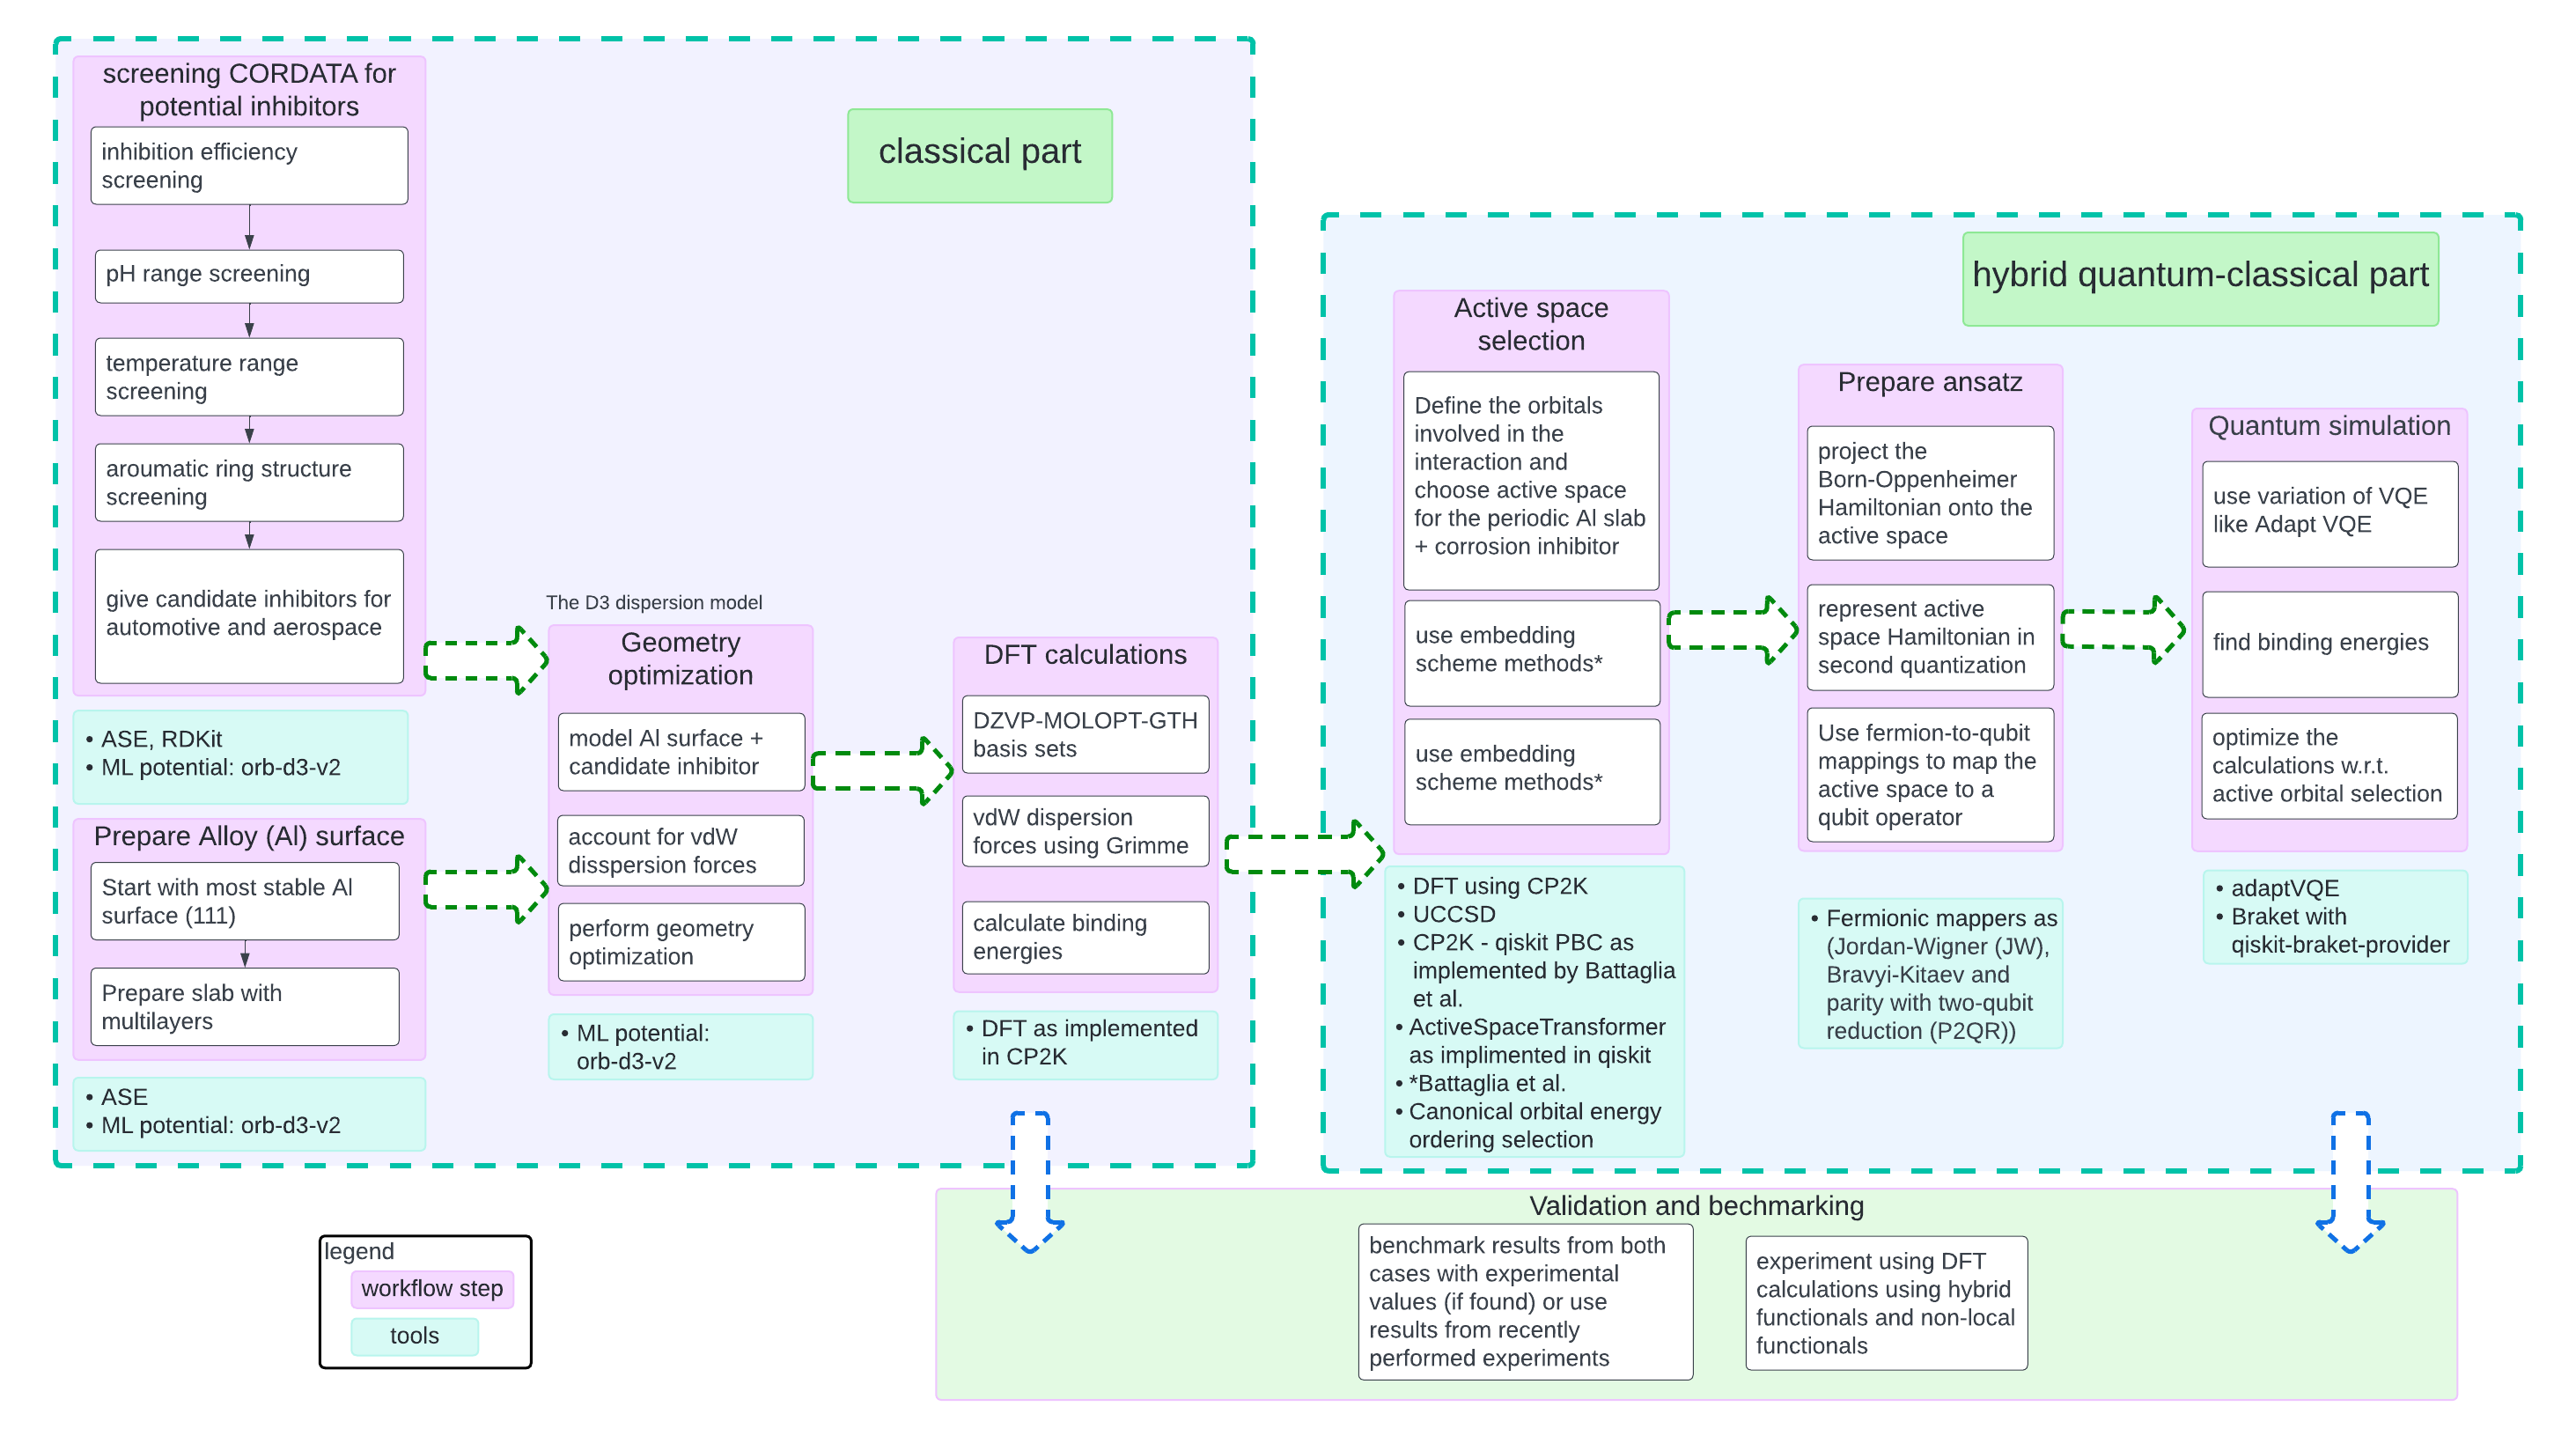
\includegraphics[width=0.95\textwidth]{../../../content/img/matsci_qc_simple_hybrid_wf.png}
\end{frame}

\begin{frame}
\frametitle{Workflow with Example System}
\centering
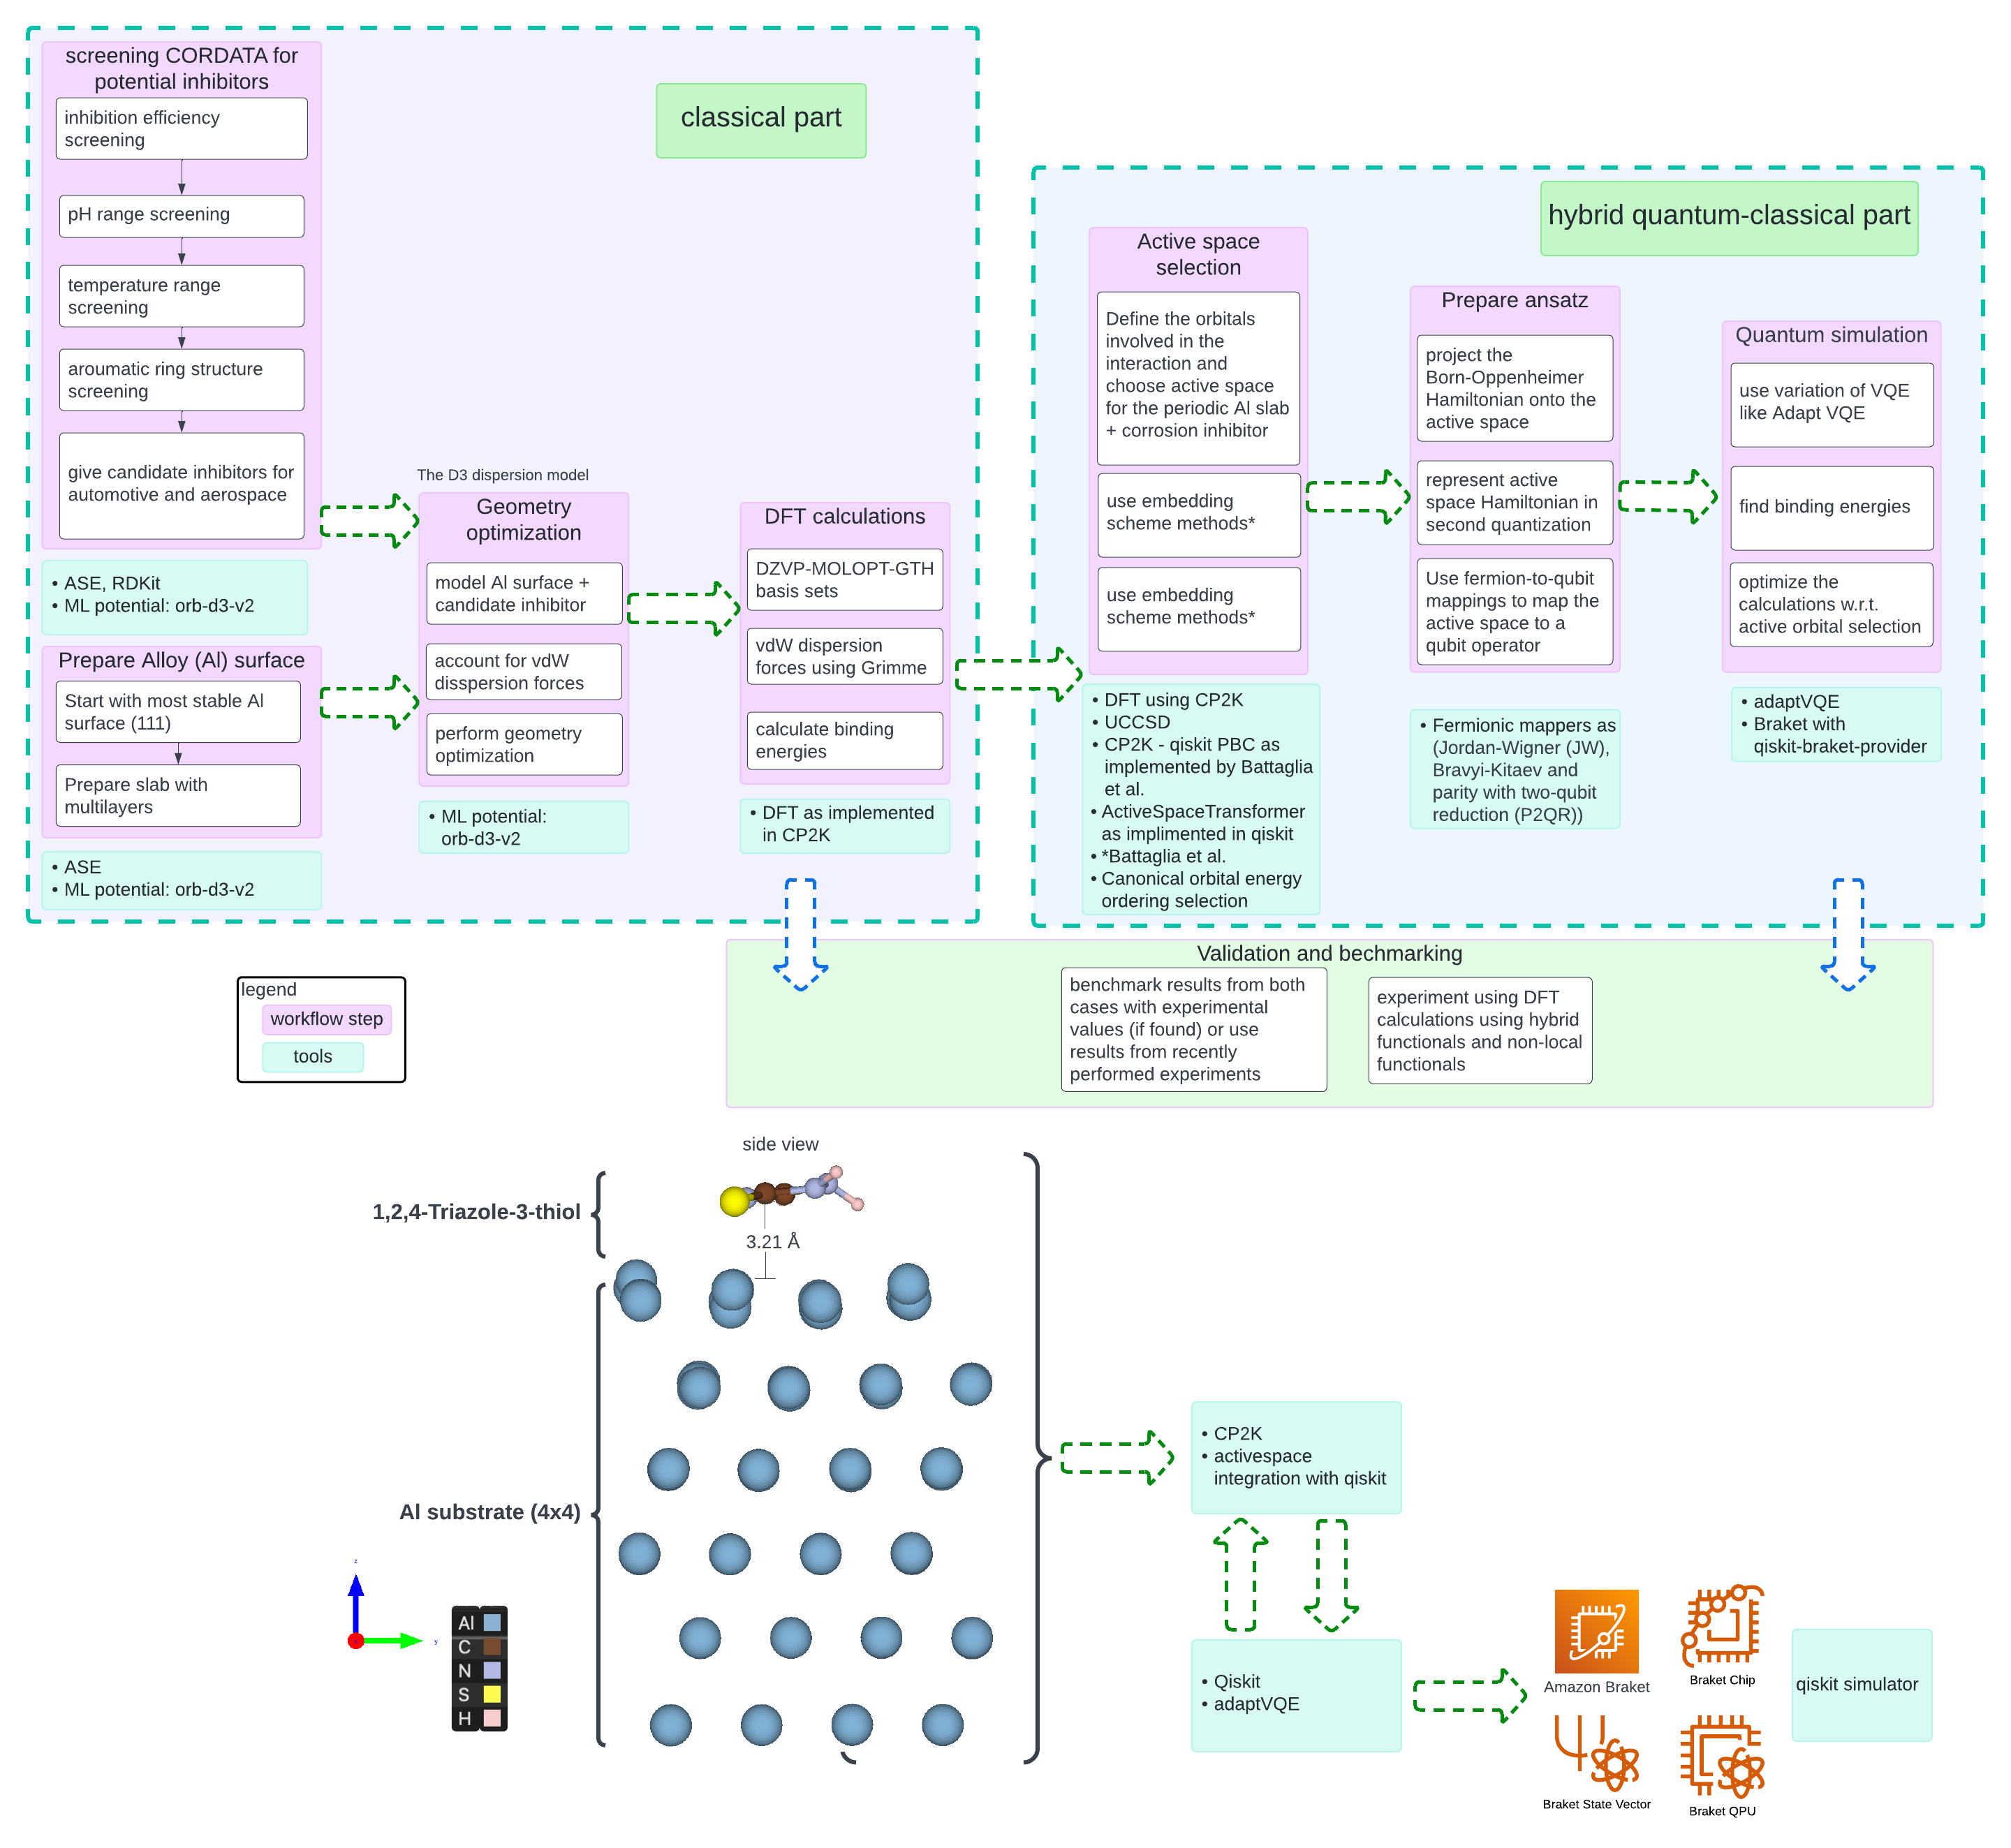
\includegraphics[width=0.65\textwidth]{../../../content/img/matsci_qc_simple_hybrid_wf_with_example.png}
\end{frame}

\begin{frame}
\frametitle{Problem Simplification}
\begin{figure}
\centering
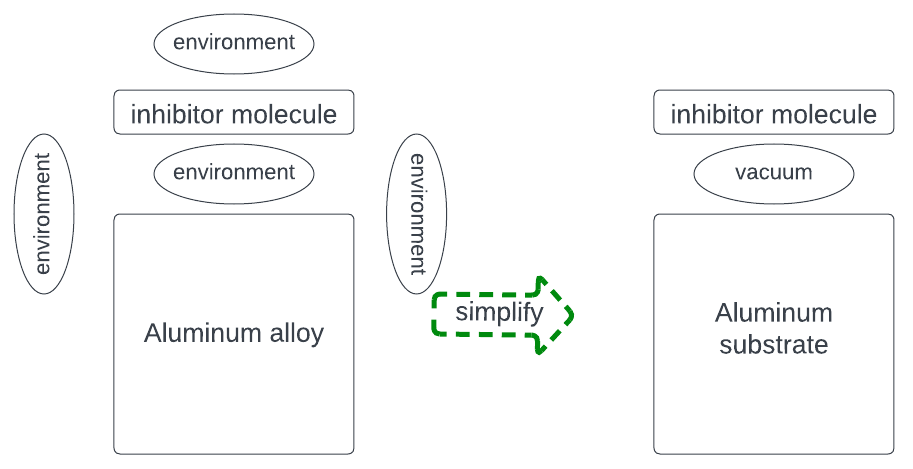
\includegraphics[width=0.95\textwidth]{../../../content/img/matsci_qc_simplify_problem.png}
\caption{Simplifying the system from alloy to pure aluminum substrate}
\end{figure}
\end{frame}

\begin{frame}
\frametitle{Research Goals}
\begin{itemize}
    \item Demonstrate hybrid quantum-classical calculations for materials
    \item Study binding energy of inhibitor molecules on metal surfaces
    \item Compare classical DFT with quantum-enhanced calculations
    \item Establish workflow for quantum-centric supercomputing
\end{itemize}
\end{frame} 